\documentclass[12pt,a4paper]{article}
\usepackage{amsmath, amssymb, geometry, booktabs, xcolor, hyperref,
            listings, pgfplots, tcolorbox, enumitem, fancyhdr, tikz, array}
\usepgfplotslibrary{fillbetween}
\geometry{margin=2.5cm}
\pgfplotsset{compat=1.18}
\tcbuselibrary{skins, breakable}

% Define custom environments
\newtcolorbox{curiositybox}[1]{colback=yellow!10, colframe=orange!80, title=#1, breakable}
\newtcolorbox{infobox}[1]{colback=blue!5, colframe=blue!60, title=#1, breakable}
\newtcolorbox{mistakebox}[1]{colback=red!5, colframe=red!60, title=#1, breakable}
\newtcolorbox{learnbox}[1]{colback=green!5, colframe=green!60, title=#1, breakable}

% Header and Footer
\pagestyle{fancy}
\fancyhf{}
\lhead{Mean Value Theorems}
\rhead{Unit 3 -- LAC}
\cfoot{\thepage}

% Document Title Setup
\title{\textbf{Mean Value Theorems} \\ \large Unit 3 -- Single Variable Calculus and Series Expansions}
\author{Department of Mathematics}
\date{\today}

\begin{document}

\maketitle
\tableofcontents
\newpage

%==============================================================================
\section{Real-World Engineering Hook}
%==============================================================================

\begin{curiositybox}{Why Should an Engineer Care?}
Imagine a vehicle undergoing crash safety testing on a straight track. A data acquisition system records
the vehicle's velocity at time $t = 0\,\text{s}$ as $v_0 = 0\,\text{m/s}$ and at $t = 10\,\text{s}$ as
$v_{10} = 120\,\text{m/s}$. The average acceleration over the interval is
$\bar{a} = (120 - 0)/10 = 12\,\text{m/s}^2$.

The \textbf{Mean Value Theorems} (MVTs) provide a rigorous mathematical guarantee:
\emph{there must exist at least one instant $c \in (0, 10)$ at which the instantaneous acceleration
equals exactly $12\,\text{m/s}^2$}. This is not intuition --- it is a proved theorem.

Engineers rely on this guarantee in three critical scenarios:
\begin{itemize}
  \item \textbf{Crash safety and structural fatigue analysis:} Peak stress in a beam under cyclic load
        equals the average stress at some specific cross-section. Identifying $c$ locates the
        fatigue-failure hot-spot. Ignoring MVT conditions and assuming a smooth stress distribution
        without verifying continuity and differentiability of the stress function leads to dangerous
        under-design.
  \item \textbf{Servo-control system design:} A PID controller uses error derivatives. If a designer
        assumes the instantaneous error rate always equals the sampled average rate without MVT
        justification, the closed-loop system can exhibit unpredicted overshoot --- sometimes causing
        irreversible actuator damage.
  \item \textbf{GPS satellite orbit correction:} Trajectory corrections compute average orbital velocity
        between two telemetry windows. Cauchy's MVT guarantees the existence of a correction instant
        where the instantaneous velocity ratio matches the average, enabling precise thruster-burst
        scheduling. Skipping the CMVT hypothesis check (in particular $g'(c) \neq 0$) leads to
        division-by-zero singularities in the navigation equations.
\end{itemize}

The root cause of every failure above is the same: applying the conclusion of an MVT without
verifying its hypotheses. This lecture note trains you to \emph{check conditions first, then conclude}.
\end{curiositybox}

%==============================================================================
\section{Why This Topic Exists}
%==============================================================================

Mean Value Theorems bridge the gap between local behaviour (derivatives) and global behaviour
(function values over an interval). They are the backbone of error estimates in numerical methods,
convergence proofs in optimisation, and the derivation of L'H\^{o}pital's Rule.

\begin{center}
\begin{tabular}{>{\bfseries}p{4.2cm} p{9.5cm}}
\toprule
Theoretical Concept & Engineering Application / Consequence of Misunderstanding \\
\midrule
Rolle's Theorem &
  Guarantees a stationary point (horizontal tangent) between two equal function values.
  Misapplication --- failing to verify $f(a)=f(b)$ or continuity --- leads to false claims of
  local minima/maxima in structural optimisation, causing over-designed or under-designed components. \\
\addlinespace
Lagrange's Mean Value Theorem (LMVT) &
  Guarantees that instantaneous rate equals average rate at some interior point.
  Skipping this in control system design produces overshoot prediction errors; in
  numerical differentiation it underlies the truncation-error bound
  $|f'(c) - \text{finite-difference}| \leq Mh$ used in all finite-element solvers. \\
\addlinespace
Cauchy's Mean Value Theorem (CMVT) &
  Underpins the rigorous proof of L'H\^{o}pital's Rule, which engineers use constantly
  in limit analysis of circuit impedances and structural buckling loads. Applying L'H\^{o}pital
  without the CMVT condition $g'(c) \neq 0$ produces undefined or incorrect limit values. \\
\bottomrule
\end{tabular}
\end{center}

\begin{learnbox}{Core Learning Objectives}
By the end of this lecture note you will be able to:
\begin{itemize}
  \item State the hypotheses and conclusion of each of Rolle's Theorem, LMVT, and CMVT precisely.
  \item Verify every hypothesis algebraically before applying any theorem.
  \item Locate the guaranteed point $c$ for polynomial, trigonometric, and mixed functions.
  \item Interpret each theorem geometrically (horizontal tangent, parallel secant--tangent, parametric ratio).
  \item Explain how Rolle's Theorem is a special case of LMVT, and how LMVT is a special case of CMVT.
  \item Apply the workflow correctly in examination problems without missing any step.
\end{itemize}
\end{learnbox}

%==============================================================================
\section{Intuition First \& Mathematical Definitions}
%==============================================================================

\subsection{Rolle's Theorem}

Picture a ball thrown upward and caught at the \emph{same height} from which it was thrown.
At some moment between release and catch the ball is momentarily stationary --- its velocity is zero.
Rolle's Theorem makes this physical intuition mathematically rigorous: if a smooth curve starts and
ends at the same height, its tangent must be horizontal somewhere in between.

\begin{infobox}{Rolle's Theorem --- Statement, Conditions, and Geometry}
\textbf{Hypotheses (all three must hold):}
\begin{enumerate}
  \item $f$ is \textbf{continuous} on the closed interval $[a, b]$.
  \item $f$ is \textbf{differentiable} on the open interval $(a, b)$.
  \item $f(a) = f(b)$ \quad (equal endpoint values).
\end{enumerate}

\textbf{Conclusion:} There exists at least one point $c \in (a, b)$ such that
\[
  f'(c) = 0.
\]

\textbf{Geometric Interpretation:} The curve $y = f(x)$ has a \emph{horizontal tangent} at
$x = c$. Equivalently, the tangent line at $(c, f(c))$ is parallel to the $x$-axis (which is
also the secant joining $(a, f(a))$ and $(b, f(b))$, since $f(a) = f(b)$).

\textbf{Proof Sketch:}
By the Extreme Value Theorem, $f$ attains its maximum $M$ and minimum $m$ on $[a, b]$.
If $M = m$, then $f$ is constant and $f'(x) = 0$ everywhere.
Otherwise, at least one of the extrema occurs at an interior point $c \in (a, b)$
(because $f(a) = f(b)$ means equal-valued endpoints cannot \emph{both} be the unique
extreme). At an interior extremum, differentiability forces $f'(c) = 0$. $\square$

\textbf{Important:} All three conditions are necessary. A counterexample when
$f(a) \neq f(b)$: $f(x) = x$ on $[0,1]$; $f'(x) = 1 \neq 0$ everywhere --- no horizontal tangent.
A counterexample when differentiability fails: $f(x) = |x|$ on $[-1, 1]$; $f(-1) = f(1) = 1$
but $f'(0)$ does not exist and indeed $f'(x) = \pm 1 \neq 0$ wherever it exists.
\end{infobox}

\textbf{Worked Example 1 (Rolle's Theorem):}

\medskip
\noindent\textbf{Problem:} Verify the conditions of Rolle's Theorem for
$f(x) = x^2 - 5x + 6$ on $[2, 3]$, and find all values of $c$ guaranteed by the theorem.

\medskip
\textbf{Step 1 --- Check continuity on $[2,3]$:}
$f(x) = x^2 - 5x + 6$ is a polynomial. Every polynomial is continuous everywhere.
Therefore $f$ is continuous on $[2, 3]$. \checkmark

\textbf{Step 2 --- Check differentiability on $(2,3)$:}
$f'(x) = 2x - 5$, which exists for all $x \in \mathbb{R}$, hence on $(2, 3)$. \checkmark

\textbf{Step 3 --- Check $f(a) = f(b)$:}
\[
  f(2) = (2)^2 - 5(2) + 6 = 4 - 10 + 6 = 0,
\]
\[
  f(3) = (3)^2 - 5(3) + 6 = 9 - 15 + 6 = 0.
\]
$f(2) = f(3) = 0$. \checkmark

\textbf{Step 4 --- Locate $c$:} Solve $f'(c) = 0$:
\[
  2c - 5 = 0 \implies c = \frac{5}{2} = 2.5.
\]

\textbf{Step 5 --- Confirm $c \in (2, 3)$:}
$2 < 2.5 < 3$. \checkmark

\textbf{Conclusion:} All three hypotheses are satisfied. Rolle's Theorem guarantees (and we
found) $c = 2.5 \in (2, 3)$ where the tangent to $f$ is horizontal.

\begin{learnbox}{Key Takeaway --- Rolle's Theorem}
The point $c = 5/2$ is the vertex of the parabola $f(x) = x^2 - 5x + 6$.
Geometrically, the parabola dips to zero at $x=2$ and $x=3$ (the roots), and its
horizontal tangent occurs exactly halfway between the roots --- confirming Rolle's Theorem.
\end{learnbox}

%----------------------------------------------------------------------
\subsection{Lagrange's Mean Value Theorem (LMVT)}

Think of a road trip: you drive $180\,\text{km}$ in $3\,\text{hours}$, giving an average speed
of $60\,\text{km/h}$. Unless you drove at a perfectly constant speed the whole time, your
speedometer must have read \emph{exactly} $60\,\text{km/h}$ at some moment. LMVT makes this
legally and mathematically guaranteed.

\begin{infobox}{Lagrange's Mean Value Theorem --- Statement, Conditions, and Geometry}
\textbf{Hypotheses:}
\begin{enumerate}
  \item $f$ is \textbf{continuous} on the closed interval $[a, b]$.
  \item $f$ is \textbf{differentiable} on the open interval $(a, b)$.
\end{enumerate}

\textbf{Conclusion:} There exists at least one point $c \in (a, b)$ such that
\[
  \boxed{f'(c) = \frac{f(b) - f(a)}{b - a}.}
\]

\textbf{Geometric Interpretation:}
The right-hand side is the \emph{slope of the secant line} joining $(a, f(a))$ and $(b, f(b))$.
LMVT guarantees that the \emph{tangent} to $y = f(x)$ at $x = c$ is \textbf{parallel} to
this secant line.

\textbf{Relationship to Rolle's Theorem:}
Rolle's Theorem is the special case of LMVT where $f(a) = f(b)$:
\[
  f'(c) = \frac{f(b) - f(a)}{b - a} = \frac{0}{b-a} = 0.
\]
Thus LMVT strictly generalises Rolle's Theorem. Indeed, the standard proof of LMVT
applies Rolle's Theorem to the auxiliary function
$h(x) = f(x) - f(a) - \dfrac{f(b)-f(a)}{b-a}(x-a)$,
which satisfies $h(a)=h(b)=0$.

\textbf{Engineering Significance:}
In numerical analysis, LMVT gives the \emph{mean-value form of the truncation error}:
for a finite-difference approximation $f'(x) \approx [f(x+h)-f(x)]/h$, the error is
$f'(c) - f'(x) = \frac{h}{2}f''(\xi)$ for some $\xi$ --- a direct consequence of LMVT.
\end{infobox}

\textbf{Worked Example 2 (LMVT):}

\medskip
\noindent\textbf{Problem:} Verify the conditions of LMVT for
$f(x) = x^3 - x^2 - x + 1$ on $[0, 2]$,
find all values of $c$, and discuss multiple solutions.

\medskip
\textbf{Step 1 --- Continuity on $[0,2]$:}
$f$ is a polynomial, continuous everywhere. \checkmark

\textbf{Step 2 --- Differentiability on $(0,2)$:}
$f'(x) = 3x^2 - 2x - 1$, exists for all $x$. \checkmark

\textbf{Step 3 --- Compute the average slope:}
\[
  f(0) = 0 - 0 - 0 + 1 = 1,
\]
\[
  f(2) = 8 - 4 - 2 + 1 = 3.
\]
\[
  k = \frac{f(2) - f(0)}{2 - 0} = \frac{3 - 1}{2} = \frac{2}{2} = 1.
\]

\textbf{Step 4 --- Solve $f'(c) = k$:}
\[
  3c^2 - 2c - 1 = 1
\]
\[
  3c^2 - 2c - 2 = 0.
\]
Using the quadratic formula:
\[
  c = \frac{2 \pm \sqrt{4 + 24}}{6} = \frac{2 \pm \sqrt{28}}{6} = \frac{2 \pm 2\sqrt{7}}{6} = \frac{1 \pm \sqrt{7}}{3}.
\]

\textbf{Step 5 --- Confirm $c \in (0,2)$:}

$\sqrt{7} \approx 2.6458$.
\[
  c_1 = \frac{1 + 2.6458}{3} = \frac{3.6458}{3} \approx 1.215, \quad
  c_2 = \frac{1 - 2.6458}{3} = \frac{-1.6458}{3} \approx -0.549.
\]
$c_1 \approx 1.215 \in (0,2)$ \checkmark; \quad $c_2 \approx -0.549 \notin (0,2)$ \texttimes.

\textbf{Edge case --- multiple solutions:}
LMVT guarantees \emph{at least one} $c$; here two algebraic solutions exist but only one
lies in the interval. When a cubic has two interior solutions both in $(a,b)$, LMVT still
holds --- it guarantees existence, not uniqueness.

\textbf{Conclusion:} The unique value guaranteed is $c = (1+\sqrt{7})/3 \approx 1.215$.

\begin{learnbox}{Key Takeaway --- LMVT}
Always check \emph{all} algebraic solutions and retain only those in the open interval $(a,b)$.
Discarding out-of-interval solutions is not an error in the theorem --- it is correct application.
\end{learnbox}

%----------------------------------------------------------------------
\subsection{Cauchy's Mean Value Theorem (CMVT)}

Imagine drawing a parametric curve where $x = g(t)$ and $y = f(t)$ as $t$ runs from $a$ to $b$.
The secant line in the $xy$-plane has slope $\Delta y / \Delta x = [f(b)-f(a)]/[g(b)-g(a)]$.
CMVT says there is a moment $t = c$ where the instantaneous slope of the curve
$dy/dx = f'(c)/g'(c)$ \emph{exactly equals} the secant slope --- a generalisation of LMVT
to parametric curves.

\begin{infobox}{Cauchy's Mean Value Theorem --- Statement, Conditions, and Applications}
\textbf{Hypotheses:}
\begin{enumerate}
  \item $f$ and $g$ are both \textbf{continuous} on $[a, b]$.
  \item $f$ and $g$ are both \textbf{differentiable} on $(a, b)$.
  \item $g'(x) \neq 0$ for all $x \in (a, b)$ \quad (this also ensures $g(b) \neq g(a)$).
\end{enumerate}

\textbf{Conclusion:} There exists at least one point $c \in (a, b)$ such that
\[
  \boxed{\frac{f'(c)}{g'(c)} = \frac{f(b) - f(a)}{g(b) - g(a)}.}
\]

\textbf{Reduction to LMVT when $g(x) = x$:}
Set $g(x) = x$, so $g'(x) = 1$, $g(a) = a$, $g(b) = b$. Then CMVT gives
\[
  \frac{f'(c)}{1} = \frac{f(b) - f(a)}{b - a},
\]
which is precisely LMVT. Thus CMVT strictly generalises LMVT (and hence Rolle's Theorem).

\textbf{Application to L'H\^{o}pital's Rule:}
When evaluating $\lim_{x \to a} f(x)/g(x)$ in the $0/0$ indeterminate form,
CMVT applied on $[a, x]$ gives a point $c$ between $a$ and $x$ such that
$f(x)/g(x) = f'(c)/g'(c)$.
As $x \to a$, $c \to a$ (by the squeeze), so
$\lim_{x\to a} f(x)/g(x) = \lim_{c \to a} f'(c)/g'(c) = \lim_{x \to a} f'(x)/g'(x)$,
which is L'H\^{o}pital's Rule. This is why engineers can apply L'H\^{o}pital
routinely: CMVT underpins its correctness.

\textbf{Geometric Interpretation (Parametric):}
On the parametric curve $(g(t), f(t))$, the secant direction from $t=a$ to $t=b$ is
$(g(b)-g(a),\; f(b)-f(a))$. CMVT guarantees a $t=c$ where the tangent direction
$(g'(c), f'(c))$ is \emph{parallel} to this secant.
\end{infobox}

\textbf{Worked Example 3 (CMVT):}

\medskip
\noindent\textbf{Problem:} Apply CMVT to $f(x) = \sin x$ and $g(x) = \cos x$ on
$[0,\, \pi/6]$. Find the point $c$ and interpret the result in terms of phase
relationships in signal processing.

\medskip
\textbf{Step 1 --- Continuity on $[0, \pi/6]$:}
$\sin x$ and $\cos x$ are continuous everywhere. \checkmark

\textbf{Step 2 --- Differentiability on $(0, \pi/6)$:}
$f'(x) = \cos x$, $g'(x) = -\sin x$. Both exist everywhere. \checkmark

\textbf{Step 3 --- Check $g'(x) \neq 0$ on $(0, \pi/6)$:}
$g'(x) = -\sin x = 0$ only when $x = 0, \pi, 2\pi, \ldots$. Since $0 < x < \pi/6 < \pi$,
we have $-\sin x < 0 \neq 0$ throughout $(0, \pi/6)$. \checkmark

\textbf{Step 4 --- Compute endpoint values:}
\[
  f(0) = \sin 0 = 0, \quad f\!\left(\frac{\pi}{6}\right) = \sin\frac{\pi}{6} = \frac{1}{2}.
\]
\[
  g(0) = \cos 0 = 1, \quad g\!\left(\frac{\pi}{6}\right) = \cos\frac{\pi}{6} = \frac{\sqrt{3}}{2}.
\]

\textbf{Step 5 --- Set up the CMVT equation:}
\[
  \frac{f(\pi/6) - f(0)}{g(\pi/6) - g(0)} = \frac{\tfrac{1}{2} - 0}{\tfrac{\sqrt{3}}{2} - 1}
  = \frac{\tfrac{1}{2}}{\tfrac{\sqrt{3}-2}{2}} = \frac{1}{\sqrt{3}-2}.
\]
Rationalise:
\[
  \frac{1}{\sqrt{3}-2} \cdot \frac{\sqrt{3}+2}{\sqrt{3}+2} = \frac{\sqrt{3}+2}{3-4} = -(\sqrt{3}+2).
\]
So the right-hand side equals $-(\sqrt{3}+2) \approx -(1.732+2) = -3.732$.

\textbf{Step 6 --- Solve for $c$:}
\[
  \frac{f'(c)}{g'(c)} = \frac{\cos c}{-\sin c} = -\cot c = -(\sqrt{3}+2).
\]
\[
  \cot c = \sqrt{3}+2 \implies \tan c = \frac{1}{\sqrt{3}+2} = \frac{\sqrt{3}-2}{(\sqrt{3})^2-4} = \frac{\sqrt{3}-2}{-1} = 2-\sqrt{3}.
\]
\[
  c = \arctan(2 - \sqrt{3}).
\]
Note that $\tan(15^\circ) = \tan(\pi/12) = 2 - \sqrt{3}$. Therefore:
\[
  c = \frac{\pi}{12} \approx 0.2618 \;\text{rad}.
\]

\textbf{Step 7 --- Confirm $c \in (0, \pi/6)$:}
$\pi/12 \approx 0.2618$ and $\pi/6 \approx 0.5236$. So $0 < \pi/12 < \pi/6$. \checkmark

\textbf{Signal Processing Interpretation:}
In a sinusoidal signal processing context, $\sin x$ and $\cos x$ represent two channels
with a $\pi/2$ phase difference. CMVT guarantees that at $c = \pi/12$ (i.e., at a
$15^\circ$ phase angle), the ratio of instantaneous rates of change equals the ratio of
cumulative changes over $[0, \pi/6]$. Engineers use this to calibrate phase-locked loops:
the ``average'' phase relationship between two oscillator signals is matched by an
instantaneous relationship at a specific angle, enabling precise synchronisation.

\begin{learnbox}{Key Takeaway --- CMVT}
CMVT requires verifying three conditions for \emph{both} functions. The condition
$g'(x) \neq 0$ is frequently overlooked by students --- always check it explicitly
over the entire open interval, not just at the endpoints.
\end{learnbox}

%==============================================================================
\section{Visual Artifacts \& Geometric Interpretation}
%==============================================================================

\subsection*{Figure 1: Rolle's Theorem --- Horizontal Tangent at $c=2$}

\begin{center}
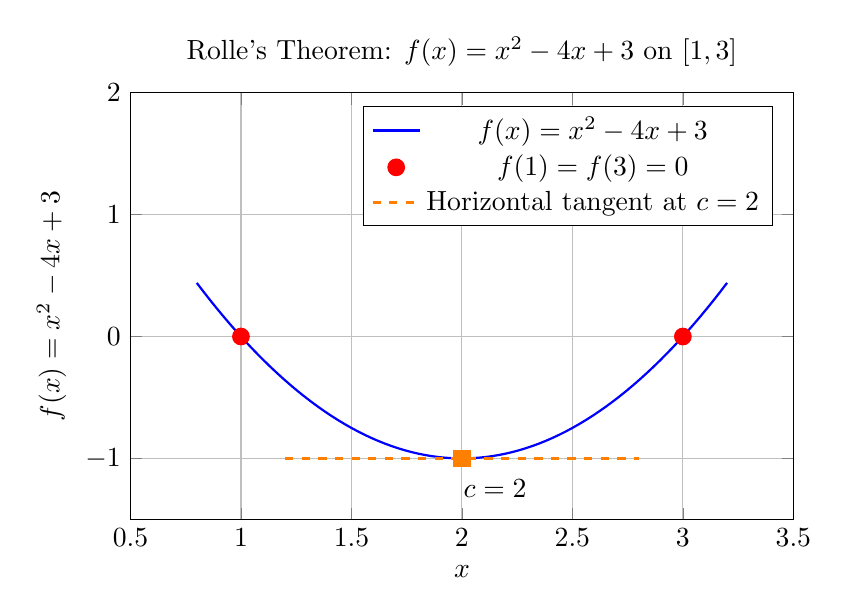
\begin{tikzpicture}
\begin{axis}[
  xlabel={$x$},
  ylabel={$f(x) = x^2 - 4x + 3$},
  xmin=0.5, xmax=3.5,
  ymin=-1.5, ymax=2,
  grid=major,
  width=10cm, height=7cm,
  title={Rolle's Theorem: $f(x)=x^2-4x+3$ on $[1,3]$},
  legend pos=north east
]
\addplot[blue, thick, domain=0.8:3.2, samples=80] {x^2 - 4*x + 3};
\addlegendentry{$f(x)=x^2-4x+3$}
% Mark f(1)=0 and f(3)=0
\addplot[only marks, mark=*, mark size=3pt, red] coordinates {(1,0) (3,0)};
\addlegendentry{$f(1)=f(3)=0$}
% Horizontal tangent at c=2
\addplot[orange, thick, dashed, domain=1.2:2.8] {-1};
\addlegendentry{Horizontal tangent at $c=2$}
% Mark c=2, f(2)=-1
\addplot[only marks, mark=square*, mark size=3pt, orange] coordinates {(2,-1)};
\node at (axis cs:2.15,-1.25) {$c=2$};
\end{axis}
\end{tikzpicture}
\end{center}

\noindent
The graph shows $f(x) = x^2 - 4x + 3$ on $[1,3]$. Both endpoints evaluate to zero
($f(1)=f(3)=0$), satisfying the equal-values condition. The horizontal tangent (orange dashed)
touches the parabola at the vertex $c=2$, where $f'(2) = 2(2)-4 = 0$.

\subsection*{Figure 2: LMVT --- Parallel Secant and Tangent for $f(x)=x^3$ on $[0,2]$}

\begin{center}
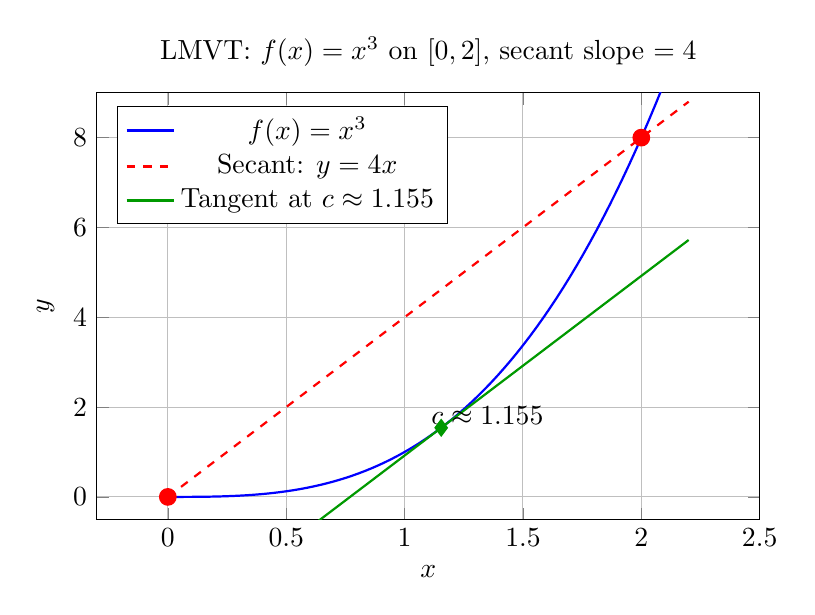
\begin{tikzpicture}
\begin{axis}[
  xlabel={$x$},
  ylabel={$y$},
  xmin=-0.3, xmax=2.5,
  ymin=-0.5, ymax=9,
  grid=major,
  width=10cm, height=7cm,
  title={LMVT: $f(x)=x^3$ on $[0,2]$, secant slope $= 4$},
  legend pos=north west
]
\addplot[blue, thick, domain=0:2.2, samples=80] {x^3};
\addlegendentry{$f(x)=x^3$}
% Secant line through (0,0) and (2,8): slope = 4
\addplot[red, dashed, thick, domain=0:2.2] {4*x};
\addlegendentry{Secant: $y=4x$}
% c = sqrt(4/3) approx 1.1547
% f(c) = c^3 approx 1.5396
% Tangent at c: y = f(c) + f'(c)(x-c) = c^3 + 3c^2*(x-c) = c^3+3c^2*x - 3c^3 = 3c^2*x - 2c^3
% c=sqrt(4/3): 3c^2=4, 2c^3=2*(4/3)^(3/2)
% numerically: c=1.1547, f(c)=1.5396, tangent: y = 4x + (1.5396 - 4*1.1547) = 4x - 3.0792
\addplot[green!60!black, thick, domain=0.2:2.2] {4*x - 3.0792};
\addlegendentry{Tangent at $c\approx1.155$}
% Mark c
\addplot[only marks, mark=diamond*, mark size=3pt, green!60!black] coordinates {(1.1547, 1.5396)};
\node at (axis cs:1.35, 1.8) {$c\approx1.155$};
% Mark endpoints
\addplot[only marks, mark=*, mark size=3pt, red] coordinates {(0,0) (2,8)};
\end{axis}
\end{tikzpicture}
\end{center}

\noindent
The secant joining $(0,0)$ and $(2,8)$ has slope $(8-0)/(2-0)=4$. The green tangent at
$c = \sqrt{4/3} \approx 1.155$ is parallel to the red secant, visually confirming LMVT.

\subsection*{Figure 3: CMVT as a Parametric Curve}

\begin{center}
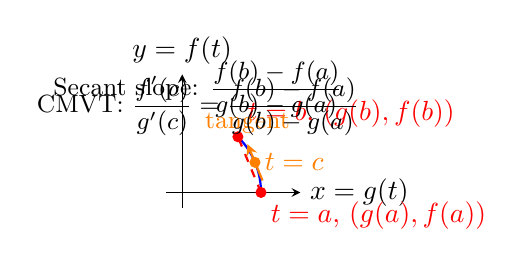
\begin{tikzpicture}[>=stealth]
% Parametric curve: x=cos(t), y=sin(t), t from 0 to pi/4 (quarter circle)
% At t=pi/8, tangent direction (-sin(pi/8), cos(pi/8))
% Secant from (cos(0),sin(0))=(1,0) to (cos(pi/4),sin(pi/4))=(sqrt2/2, sqrt2/2)
\draw[->] (-0.2,0) -- (1.5,0) node[right] {$x = g(t)$};
\draw[->] (0,-0.2) -- (0,1.5) node[above] {$y = f(t)$};
% Parametric arc
\draw[blue, thick] plot[domain=0:45, samples=50, variable=\t]
  ({cos(\t)}, {sin(\t)});
% Endpoints
\fill[red] (1,0) circle (2pt) node[below right] {$t=a$, $(g(a),f(a))$};
\fill[red] ({cos(45)},{sin(45)}) circle (2pt) node[above right] {$t=b$, $(g(b),f(b))$};
% Secant line
\draw[red, dashed, thick] (1,0) -- ({cos(45)},{sin(45)});
% Tangent at c = pi/8 = 22.5 degrees
\pgfmathsetmacro{\cx}{cos(22.5)}
\pgfmathsetmacro{\cy}{sin(22.5)}
\fill[orange] (\cx,\cy) circle (2pt) node[right] {$t=c$};
% Tangent direction: dx/dt=-sin(t), dy/dt=cos(t) at t=22.5
\pgfmathsetmacro{\tdx}{-sin(22.5)*0.25}
\pgfmathsetmacro{\tdy}{cos(22.5)*0.25}
\draw[orange, thick, ->] (\cx-\tdx, \cy-\tdy) -- (\cx+\tdx, \cy+\tdy)
  node[above] {\small tangent};
% Annotation
\node[align=left, font=\small] at (0.2, 1.3)
  {Secant slope: $\dfrac{f(b)-f(a)}{g(b)-g(a)}$};
\node[align=left, font=\small] at (0.2, 1.1)
  {CMVT: $\dfrac{f'(c)}{g'(c)} = \dfrac{f(b)-f(a)}{g(b)-g(a)}$};
\end{tikzpicture}
\end{center}

\noindent
The parametric curve (blue arc) traces $(g(t), f(t)) = (\cos t, \sin t)$ from $t=a$ to $t=b$.
The red dashed secant connects the start and end points. CMVT guarantees a point $t=c$
(orange) where the tangent direction is \emph{parallel} to the secant direction.

%==============================================================================
\section{Step-by-Step Algorithmic Workflow}
%==============================================================================

\begin{tcolorbox}[colback=gray!5, colframe=black!70, title=Algorithm: Applying Mean Value Theorems, breakable]

\textbf{WORKFLOW FOR ROLLE'S THEOREM}

\begin{enumerate}[label=\textbf{R\arabic*.}]
  \item \textbf{Check continuity on $[a,b]$:} Determine the type of $f(x)$ (polynomial,
        rational, trigonometric, etc.) and confirm it is defined and continuous on the
        closed interval. Note any points of discontinuity.
  \item \textbf{Check differentiability on $(a,b)$:} Compute $f'(x)$. Confirm it exists
        for every $x$ in the open interval. Watch for corner points (absolute value), cusps,
        or vertical tangents.
  \item \textbf{Verify $f(a) = f(b)$:} Compute both values numerically. If they differ,
        Rolle's Theorem \emph{does not apply} (but a stationary point may still exist).
  \item \textbf{Solve $f'(c) = 0$:} Set the derivative equal to zero and solve the resulting
        equation algebraically.
  \item \textbf{Confirm $c \in (a,b)$:} Evaluate each solution numerically; retain only
        those strictly between $a$ and $b$.
\end{enumerate}

\medskip
\textbf{WORKFLOW FOR LAGRANGE'S MEAN VALUE THEOREM (LMVT)}

\begin{enumerate}[label=\textbf{L\arabic*.}]
  \item \textbf{Check continuity on $[a,b]$:} Same as R1.
  \item \textbf{Check differentiability on $(a,b)$:} Same as R2.
  \item \textbf{Compute the mean slope:} Calculate $k = \dfrac{f(b)-f(a)}{b-a}$.
        This is the slope of the secant line.
  \item \textbf{Solve $f'(c) = k$:} Set the derivative equal to $k$ and solve for $c$.
  \item \textbf{Confirm $c \in (a,b)$:} Retain only solutions in the open interval.
\end{enumerate}

\medskip
\textbf{WORKFLOW FOR CAUCHY'S MEAN VALUE THEOREM (CMVT)}

\begin{enumerate}[label=\textbf{C\arabic*.}]
  \item \textbf{Check continuity of $f$ and $g$ on $[a,b]$:} Both functions must be
        continuous on the closed interval.
  \item \textbf{Check differentiability of $f$ and $g$ on $(a,b)$:} Both derivatives
        must exist throughout the open interval.
  \item \textbf{Verify $g'(x) \neq 0$ on $(a,b)$:} Find zeros of $g'(x)$; confirm none
        lie in $(a,b)$. If $g'(x_0) = 0$ for some $x_0 \in (a,b)$, CMVT does not apply.
  \item \textbf{Compute the ratio:} Calculate
        $R = \dfrac{f(b)-f(a)}{g(b)-g(a)}$.
  \item \textbf{Solve $f'(c)/g'(c) = R$:} This typically reduces to solving a
        trigonometric or algebraic equation.
  \item \textbf{Confirm $c \in (a,b)$:} Retain only solutions in the open interval.
\end{enumerate}

\end{tcolorbox}

%==============================================================================
\section{Fully Worked Step-by-Step Numerical Examples}
%==============================================================================

\subsection*{Example A: Rolle's Theorem --- Polynomial on a Symmetric Interval}

\noindent\textbf{Problem:} Apply Rolle's Theorem to $f(x) = x^3 - 6x^2 + 11x - 6$ on $[1, 3]$.

\medskip
\textbf{Step 1:} $f$ is a polynomial, continuous on $[1,3]$. \checkmark

\textbf{Step 2:} $f'(x) = 3x^2 - 12x + 11$, exists everywhere. \checkmark

\textbf{Step 3:}
\[
  f(1) = 1 - 6 + 11 - 6 = 0, \quad f(3) = 27 - 54 + 33 - 6 = 0.
\]
$f(1) = f(3) = 0$. \checkmark

\textbf{Step 4:} Solve $f'(c) = 0$:
\[
  3c^2 - 12c + 11 = 0 \implies c = \frac{12 \pm \sqrt{144 - 132}}{6} = \frac{12 \pm \sqrt{12}}{6}
  = \frac{12 \pm 2\sqrt{3}}{6} = 2 \pm \frac{\sqrt{3}}{3}.
\]
\[
  c_1 = 2 + \frac{1}{\sqrt{3}} \approx 2 + 0.577 = 2.577, \quad
  c_2 = 2 - \frac{1}{\sqrt{3}} \approx 2 - 0.577 = 1.423.
\]

\textbf{Step 5:} Both $c_1 \approx 2.577$ and $c_2 \approx 1.423$ lie in $(1,3)$. \checkmark

\textbf{Conclusion:} There are \emph{two} points in $(1,3)$ where $f'(c)=0$, namely
$c = 2 \pm 1/\sqrt{3}$. Rolle's Theorem is verified (it guarantees \emph{at least one}).

\begin{learnbox}{Insight}
$f(x) = (x-1)(x-2)(x-3)$ --- its three real roots are $1, 2, 3$. By Rolle's Theorem
applied on $[1,2]$ and $[2,3]$ separately, stationary points exist in each sub-interval.
Combining into $[1,3]$ finds both.
\end{learnbox}

\subsection*{Example B: LMVT --- Trigonometric Function}

\noindent\textbf{Problem:} Verify LMVT for $f(x) = \sin x$ on $[0, \pi/2]$ and find $c$.

\medskip
\textbf{Step 1:} $\sin x$ is continuous on $[0, \pi/2]$. \checkmark

\textbf{Step 2:} $f'(x) = \cos x$, exists everywhere. \checkmark

\textbf{Step 3:}
\[
  k = \frac{f(\pi/2) - f(0)}{\pi/2 - 0} = \frac{1 - 0}{\pi/2} = \frac{2}{\pi} \approx 0.6366.
\]

\textbf{Step 4:} Solve $f'(c) = k$:
\[
  \cos c = \frac{2}{\pi} \implies c = \arccos\!\left(\frac{2}{\pi}\right).
\]
\[
  c \approx \arccos(0.6366) \approx 0.8861 \;\text{rad} \approx 50.76^\circ.
\]

\textbf{Step 5:} $0 < 0.8861 < \pi/2 \approx 1.5708$. \checkmark

\textbf{Conclusion:} At $c = \arccos(2/\pi) \approx 0.886\,\text{rad}$, the instantaneous rate
of change of $\sin x$ equals the average rate over $[0, \pi/2]$.

\begin{learnbox}{Engineering Relevance}
In electrical engineering, $\sin x$ models the voltage waveform.
The average value of $|\sin x|$ over a half-cycle is $2/\pi \approx 0.637$ times the peak,
the well-known rectified-average formula. LMVT confirms there is a phase angle where
the instantaneous slope equals this normalised average.
\end{learnbox}

\subsection*{Example C: CMVT Applied to Exponential Functions}

\noindent\textbf{Problem:} Apply CMVT with $f(x) = e^{2x}$ and $g(x) = e^x$ on $[0, 1]$.
Find $c$ and relate the result to a limit comparison.

\medskip
\textbf{Step 1:} Both $e^{2x}$ and $e^x$ are continuous on $[0,1]$. \checkmark

\textbf{Step 2:} $f'(x) = 2e^{2x}$, $g'(x) = e^x$. Both exist everywhere. \checkmark

\textbf{Step 3:} $g'(x) = e^x > 0$ for all $x$, so $g'(x) \neq 0$ on $(0,1)$. \checkmark

\textbf{Step 4:}
\[
  f(0) = e^0 = 1, \quad f(1) = e^2 \approx 7.389,
\]
\[
  g(0) = e^0 = 1, \quad g(1) = e^1 = e \approx 2.718.
\]
\[
  R = \frac{f(1)-f(0)}{g(1)-g(0)} = \frac{e^2 - 1}{e - 1}.
\]
Numerically: $R = (7.389 - 1)/(2.718 - 1) = 6.389/1.718 \approx 3.719$.

\textbf{Step 5:} Solve $f'(c)/g'(c) = R$:
\[
  \frac{2e^{2c}}{e^c} = \frac{e^2 - 1}{e - 1} \implies 2e^c = \frac{e^2-1}{e-1}.
\]
Note $e^2-1 = (e-1)(e+1)$, so:
\[
  2e^c = e+1 \implies e^c = \frac{e+1}{2} \implies c = \ln\!\left(\frac{e+1}{2}\right).
\]
\[
  c = \ln\!\left(\frac{2.718+1}{2}\right) = \ln(1.859) \approx 0.620.
\]

\textbf{Step 6:} $0 < 0.620 < 1$. \checkmark

\textbf{Limit interpretation:}
As $x \to 0$, $f(x)/g(x) = e^{2x}/e^x = e^x \to 1$. L'H\^{o}pital (backed by CMVT) gives
$f'(x)/g'(x) = 2e^{2x}/e^x = 2e^x \to 2$, showing the limit of the \emph{ratio of rates}
differs from the limit of the ratio itself --- illustrating when and how CMVT/L'H\^{o}pital
applies.

\begin{learnbox}{Key Takeaway --- CMVT Example}
The elegant simplification $e^2 - 1 = (e-1)(e+1)$ yielded a clean closed-form for $c$.
Always factor before resorting to numerical methods --- algebraic manipulation often produces
the exact answer required in examinations.
\end{learnbox}

%==============================================================================
\section{Tabular Comparison \& Workflow Reference}
%==============================================================================

\begin{center}
\begin{tabular}{>{\bfseries}p{3.5cm} p{3.5cm} p{3.5cm} p{4cm}}
\toprule
Property & Rolle's Theorem & LMVT & CMVT \\
\midrule
Hypotheses &
  $f$ cont.\ on $[a,b]$; diff.\ on $(a,b)$; $f(a)=f(b)$ &
  $f$ cont.\ on $[a,b]$; diff.\ on $(a,b)$ &
  $f,g$ cont.\ on $[a,b]$; $f,g$ diff.\ on $(a,b)$; $g'(x)\neq0$ \\
\addlinespace
Conclusion &
  $\exists\, c \in (a,b)$: $f'(c)=0$ &
  $\exists\, c \in (a,b)$: $f'(c) = \dfrac{f(b)-f(a)}{b-a}$ &
  $\exists\, c \in (a,b)$: $\dfrac{f'(c)}{g'(c)} = \dfrac{f(b)-f(a)}{g(b)-g(a)}$ \\
\addlinespace
Special Case Of &
  (most restrictive) &
  Generalisation of Rolle's &
  Generalisation of LMVT \\
\addlinespace
Geometric Meaning &
  Horizontal tangent at $c$ &
  Tangent at $c$ is parallel to secant $AB$ &
  Tangent to parametric curve is parallel to parametric secant \\
\addlinespace
Key Equation to Solve &
  $f'(c)=0$ &
  $f'(c)=\dfrac{f(b)-f(a)}{b-a}$ &
  $f'(c) \cdot [g(b)-g(a)] = g'(c) \cdot [f(b)-f(a)]$ \\
\addlinespace
Primary Engineering Use &
  Locate stationary points; optimisation; root-bounding &
  Average vs.\ instantaneous rate; numerical truncation error &
  L'H\^{o}pital's Rule; parametric trajectory analysis; phase comparison \\
\addlinespace
Extra Condition &
  Equal endpoint values: $f(a)=f(b)$ &
  None beyond continuity and differentiability &
  $g'(x)\neq0$ throughout $(a,b)$; also ensures $g(b)\neq g(a)$ \\
\bottomrule
\end{tabular}
\end{center}

%==============================================================================
\section{Common Student Mistakes \& Pitfalls}
%==============================================================================

\begin{mistakebox}{Common Mistakes in Mean Value Theorems}
\begin{tabular}{>{\bfseries}p{4.5cm} p{4.5cm} p{5.5cm}}
\toprule
Mistake Made & Why Students Do It & Correct Mathematical Approach \\
\midrule
Applying Rolle's Theorem without verifying $f(a)=f(b)$ &
  Endpoints look equal from a rough graph sketch; students skip algebraic computation &
  Always compute $f(a)$ and $f(b)$ explicitly with full arithmetic before claiming the condition holds \\
\addlinespace
Confusing ``continuous on $(a,b)$'' with ``continuous on $[a,b]$'' for LMVT &
  Students copy the open-interval differentiability requirement to continuity by mistake &
  Continuity is required on the \emph{closed} interval $[a,b]$; differentiability on the
  \emph{open} interval $(a,b)$ --- these are separate and both mandatory \\
\addlinespace
Using CMVT without checking $g'(x)\neq0$ &
  Students assume a smooth-looking function cannot have zero derivative &
  Explicitly set $g'(x)=0$ and solve; confirm no solution lies in $(a,b)$;
  if one does, CMVT cannot be applied directly \\
\addlinespace
Accepting $c$ values outside $(a,b)$ &
  Quadratic/trig equations yield multiple solutions; students forget to filter &
  After solving $f'(c)=k$, check \emph{every} solution: keep only those with $a < c < b$ \\
\addlinespace
Claiming the theorem guarantees a \emph{unique} $c$ &
  The statement ``there exists $c$'' is misread as ``there is exactly one $c$'' &
  MVTs guarantee \emph{at least one} $c$; polynomials of degree $n$ may yield up to $n-1$
  valid values of $c$ in $(a,b)$ \\
\addlinespace
Applying L'H\^{o}pital's Rule without verifying the indeterminate form &
  Students apply L'H\^{o}pital mechanically to every limit &
  L'H\^{o}pital (whose validity rests on CMVT) applies only when both numerator and
  denominator tend to $0$ or both tend to $\pm\infty$ at the point \\
\bottomrule
\end{tabular}
\end{mistakebox}

%==============================================================================
\section{Comprehensive Assessment Suite}
%==============================================================================

\subsection*{Viva-Voce Questions}

\begin{enumerate}
  \item \textbf{[Rolle's]} State Rolle's Theorem precisely, listing all three hypotheses.
        Construct a counterexample demonstrating that the conclusion fails when $f(a) \neq f(b)$.

  \item \textbf{[Rolle's]} Is Rolle's Theorem a special case of LMVT? Justify your answer by
        deriving Rolle's Theorem from LMVT in two lines.

  \item \textbf{[Rolle's]} For $f(x) = |x-1|$ on $[0,2]$, does Rolle's Theorem apply?
        Check each hypothesis and state which one fails and why.

  \item \textbf{[LMVT]} Explain the geometric interpretation of LMVT in terms of secant and
        tangent lines. Draw a rough sketch illustrating the result.

  \item \textbf{[LMVT]} If $f(x)$ is a constant function on $[a,b]$, what does LMVT give?
        What does this say physically about a stationary object?

  \item \textbf{[LMVT]} State the mean-value form of the numerical differentiation truncation error
        and identify the MVT result that underpins it.

  \item \textbf{[CMVT]} State Cauchy's Mean Value Theorem. Show explicitly that setting $g(x) = x$
        reduces it to LMVT.

  \item \textbf{[CMVT]} Explain how CMVT is used in the proof of L'H\^{o}pital's Rule for the
        $0/0$ indeterminate form. Which hypothesis of CMVT ensures the denominator in
        L'H\^{o}pital is non-zero?
\end{enumerate}

\subsection*{Descriptive Problems}

\begin{enumerate}
  \item \textbf{[Rolle's --- 6 marks]} Verify Rolle's Theorem for $f(x) = x(x-1)(x-3)$ on $[0,3]$.
        Find all values of $c$. Interpret geometrically by sketching the curve and marking the
        horizontal tangents.

        \textit{Hint:} Expand $f$, compute $f'(x)$, set $f'(c)=0$, solve the resulting quadratic.

  \item \textbf{[LMVT --- 6 marks]} Verify LMVT for $f(x) = \ln x$ on $[1, e]$.
        Find the exact value of $c$ and verify $c \in (1, e)$.

        \textit{Hint:} $f'(x) = 1/x$; average slope $= (\ln e - \ln 1)/(e-1) = 1/(e-1)$.

  \item \textbf{[LMVT --- 8 marks]} A train travels from station A to station B
        (distance $= 240\,\text{km}$) in $3\,\text{hours}$. Use LMVT to argue that at some
        instant the train's speedometer read exactly $80\,\text{km/h}$.
        Then model velocity as $v(t) = 80 + 40\sin(\pi t/3)$, $t \in [0,3]$,
        compute $v(0)$, $v(3)$, and find $t = c$ where $v(c) = 80$.

  \item \textbf{[CMVT --- 8 marks]} Apply CMVT to $f(x) = x^2$ and $g(x) = x^3$ on $[1,2]$.
        Verify all conditions, find $c$, and verify $c \in (1,2)$.

        \textit{Hint:} $g'(x) = 3x^2 > 0$ on $(1,2)$; solve $2c / (3c^2) = (4-1)/(8-1)$.

  \item \textbf{[Combined --- 10 marks]} State and prove LMVT using Rolle's Theorem.
        [Apply Rolle's Theorem to the auxiliary function
        $h(x) = f(x) - f(a) - \dfrac{f(b)-f(a)}{b-a}(x-a)$.]
        Then use the result to prove that if $f'(x) = 0$ for all $x \in (a,b)$,
        then $f$ is constant on $[a,b]$.
\end{enumerate}

\subsection*{Multiple Choice Questions}

\begin{enumerate}
  \item \textbf{[Rolle's]} For $f(x) = x^2 - 4$ on $[-2, 2]$, which value of $c$ is guaranteed
        by Rolle's Theorem?
        \begin{enumerate}[label=(\Alph*)]
          \item $c = 1$
          \item \textbf{$c = 0$}
          \item $c = -1$
          \item $c = 2$
        \end{enumerate}
        \textit{Explanation:} $f(-2) = 0 = f(2)$, all conditions met. $f'(c) = 2c = 0 \Rightarrow c = 0 \in (-2,2)$.

  \item \textbf{[Rolle's]} For which function does Rolle's Theorem \emph{fail} to apply on $[-1, 1]$?
        \begin{enumerate}[label=(\Alph*)]
          \item $f(x) = x^2 - 1$
          \item $f(x) = \cos(\pi x)$
          \item \textbf{$f(x) = |x|$}
          \item $f(x) = x^4 - 1$
        \end{enumerate}
        \textit{Explanation:} $|x|$ is not differentiable at $x=0 \in (-1,1)$, violating hypothesis 2.

  \item \textbf{[LMVT]} For $f(x) = x^2$ on $[1, 3]$, LMVT guarantees a point $c$ equal to:
        \begin{enumerate}[label=(\Alph*)]
          \item $c = 1.5$
          \item $c = 2.5$
          \item $c = 3$
          \item \textbf{$c = 2$}
        \end{enumerate}
        \textit{Explanation:} Mean slope $= (9-1)/(3-1) = 4$. Solve $f'(c)=2c=4 \Rightarrow c=2 \in (1,3)$.

  \item \textbf{[LMVT]} LMVT states that for $f$ continuous on $[a,b]$ and differentiable on $(a,b)$,
        there exists $c \in (a,b)$ such that:
        \begin{enumerate}[label=(\Alph*)]
          \item $f'(c) = 0$
          \item $f''(c) = 0$
          \item \textbf{$f'(c) = \dfrac{f(b)-f(a)}{b-a}$}
          \item $f(c) = \dfrac{f(a)+f(b)}{2}$
        \end{enumerate}
        \textit{Explanation:} This is the exact statement of LMVT. Option (A) is Rolle's Theorem (special case).

  \item \textbf{[CMVT]} In Cauchy's MVT applied to $f$ and $g$ on $[a,b]$, which additional
        condition beyond continuity and differentiability is required?
        \begin{enumerate}[label=(\Alph*)]
          \item $f'(x) \neq 0$ on $(a,b)$
          \item $f(a) = f(b)$
          \item \textbf{$g'(x) \neq 0$ on $(a,b)$}
          \item $g(a) = g(b)$
        \end{enumerate}
        \textit{Explanation:} CMVT requires $g'(x)\neq 0$ to ensure $g(b)\neq g(a)$ and avoid
        division by zero in the conclusion $f'(c)/g'(c) = [f(b)-f(a)]/[g(b)-g(a)]$.

  \item \textbf{[CMVT]} When $g(x) = x$ is substituted into CMVT, the result is:
        \begin{enumerate}[label=(\Alph*)]
          \item Rolle's Theorem
          \item \textbf{Lagrange's Mean Value Theorem}
          \item Taylor's Theorem
          \item L'H\^{o}pital's Rule
        \end{enumerate}
        \textit{Explanation:} With $g(x)=x$: $g'(x)=1$, $g(b)-g(a)=b-a$. CMVT becomes
        $f'(c)/1=[f(b)-f(a)]/(b-a)$, which is exactly LMVT.
\end{enumerate}

%==============================================================================
\section{Quick Recap \& Formula Sheet}
%==============================================================================

\begin{learnbox}{Mean Value Theorems --- Formula Sheet and Key Takeaways}
\begin{itemize}
  \item \textbf{Rolle's Theorem:} If $f$ is continuous on $[a,b]$, differentiable on $(a,b)$,
        and $f(a)=f(b)$, then $\exists\, c \in (a,b)$ with $f'(c)=0$
        (horizontal tangent between equal-height endpoints).
  \item \textbf{LMVT Formula:} $f'(c) = \dfrac{f(b)-f(a)}{b-a}$; the instantaneous rate at $c$
        equals the average rate over $[a,b]$ --- the ``speedometer equals average speed'' theorem.
  \item \textbf{CMVT Formula:} $\dfrac{f'(c)}{g'(c)} = \dfrac{f(b)-f(a)}{g(b)-g(a)}$;
        requires $g'(x)\neq 0$ on $(a,b)$; reduces to LMVT when $g(x)=x$.
  \item \textbf{Hierarchy:} Rolle's Theorem $\subset$ LMVT $\subset$ CMVT.
        Each is a strict generalisation of the previous.
  \item \textbf{Verification Workflow:} Always check \emph{all} hypotheses first; then solve;
        then filter solutions to retain only those in the open interval $(a,b)$.
  \item \textbf{L'H\^{o}pital's Rule} is a corollary of CMVT:
        $\lim_{x\to a}\dfrac{f(x)}{g(x)} = \lim_{x\to a}\dfrac{f'(x)}{g'(x)}$
        when both $\to 0$ or both $\to \infty$, provided the right-side limit exists.
  \item \textbf{Geometric Summary:} Rolle's $\to$ horizontal tangent;
        LMVT $\to$ tangent parallel to secant;
        CMVT $\to$ tangent parallel to parametric secant.
  \item \textbf{Engineering Guarantee:} MVTs are existence theorems --- they do not tell you
        the value of $c$, only that one exists. You must solve $f'(c)=0$ or $f'(c)=k$ or
        $f'(c)/g'(c)=R$ explicitly to find the actual value.
\end{itemize}
\end{learnbox}

\end{document}
